\section{Finite state automata}

\paragraph*{Finite state automaton}
A Finite State Automaton (FSA) comprises three fundamental components:
\begin{enumerate}
    \item The input tape, containing the input string $x \in \Sigma^{\ast}$.
    \item The control unit, equipped with finite memory containing the state table.
    \item The input head, initially positioned at the start marker of string $x$, which advances rightward with each move until it reaches the end-marker of the string or encounters an error.
\end{enumerate}
Upon reading an input character, the automaton updates its current state in the control unit.
After scanning the entire input string $x$, the automaton either recognizes or rejects the string based on its current state.

\paragraph*{State-transition graph}
The state-transition graph is a directed graph that represents the automaton and consists of the following elements:
\begin{itemize}
    \item \textit{Nodes}: represent the states of the control unit. 
    \item \textit{Arcs}: represent the moves of the automaton. 
\end{itemize}
Each arc is labeled with an input symbol and signifies a valid move when the current state matches the source state of the arc, and the current input symbol matches the arc label. 
The state-transition graph features a unique initial state but may have none, one, or more final states. 
It can be depicted using an incidence matrix, where each entry, indexed by the current state and input symbol, indicates the next state. 
This matrix is commonly known as the state table. 
Alternatively, a syntax diagram, the dual of the state-transition graph, can be employed.
\begin{example}
    Consider the language over the alphabet $\Sigma=\delta \cup \{0,\cdot\}$, where $\delta=\{1,2,3,4,5,6,7,8,9\}$ generates decimal numbers. 
    The corresponding regular expression is:
    \[e=\left( 0 \cup \delta (0 \cup \delta)^{\ast} \right) \cdot (0 \cup \delta)^{+}\]
    The associated state-transition graph and state-transition table are depicted below:
    \begin{figure}[H]
        \centering
        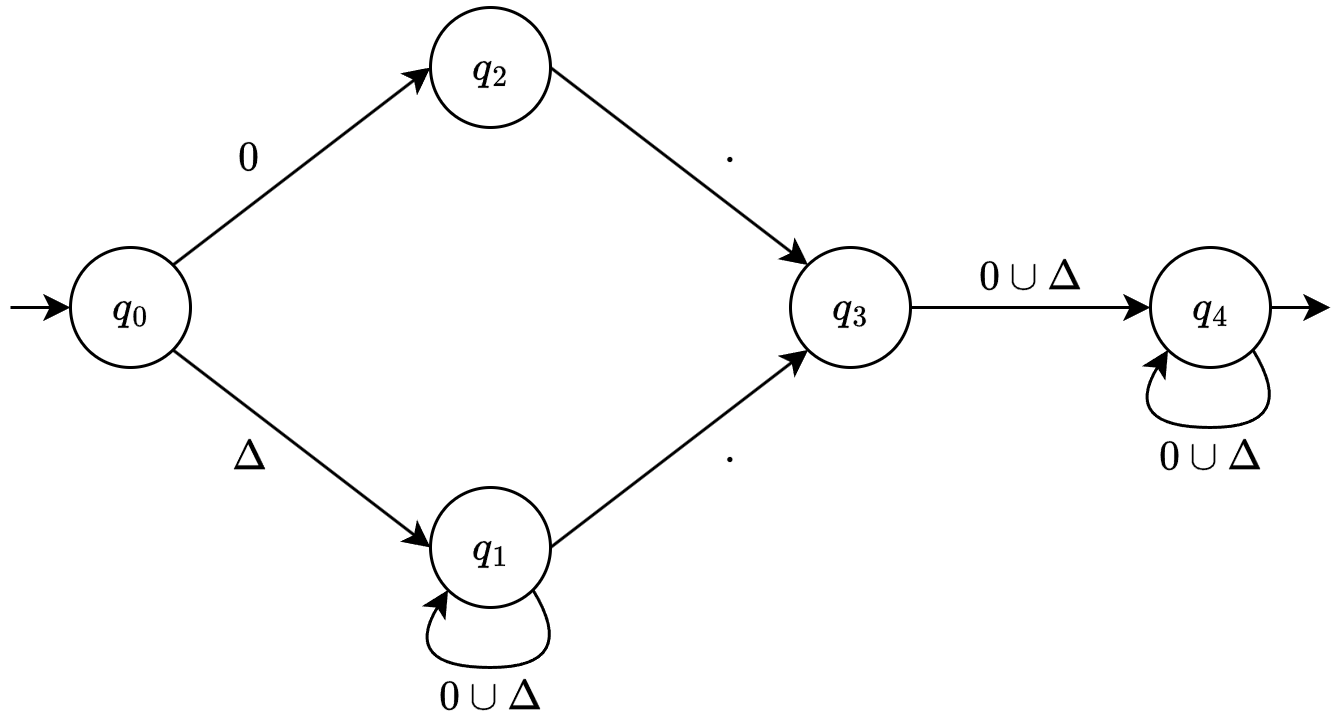
\includegraphics[width=0.75\linewidth]{images/fsa1.png}
    \end{figure}
    \begin{table}[H]
        \centering
        \begin{tabular}{|c|ccccc|}
        \hline
        \textbf{Current state} & \multicolumn{5}{c|}{\textbf{Current character}}\\ \cline {2-6}
                               & 0      & 1      & $\dots$  & 9      & $\cdot$  \\ \hline
        $\rightarrow q_0$      & $q_2$  & $q_1$  & $\dots$  & $q_1$  & -        \\
        $q_1$                  & $q_1$  & $q_1$  & $\dots$  & $q_1$  & $q_3$    \\
        $q_2$                  & -      & -      & $\dots$  & -      & $q_3$    \\
        $q_3$                  & $q_4$  & $q_4$  & $\dots$  & $q_4$  & -        \\
        $q_4 \rightarrow$      & $q_4$  & $q_4$  & $\dots$  & $q_4$  & -        \\ \hline
        \end{tabular}
    \end{table}
    The syntax diagram is:
    \begin{figure}[H]
        \centering
        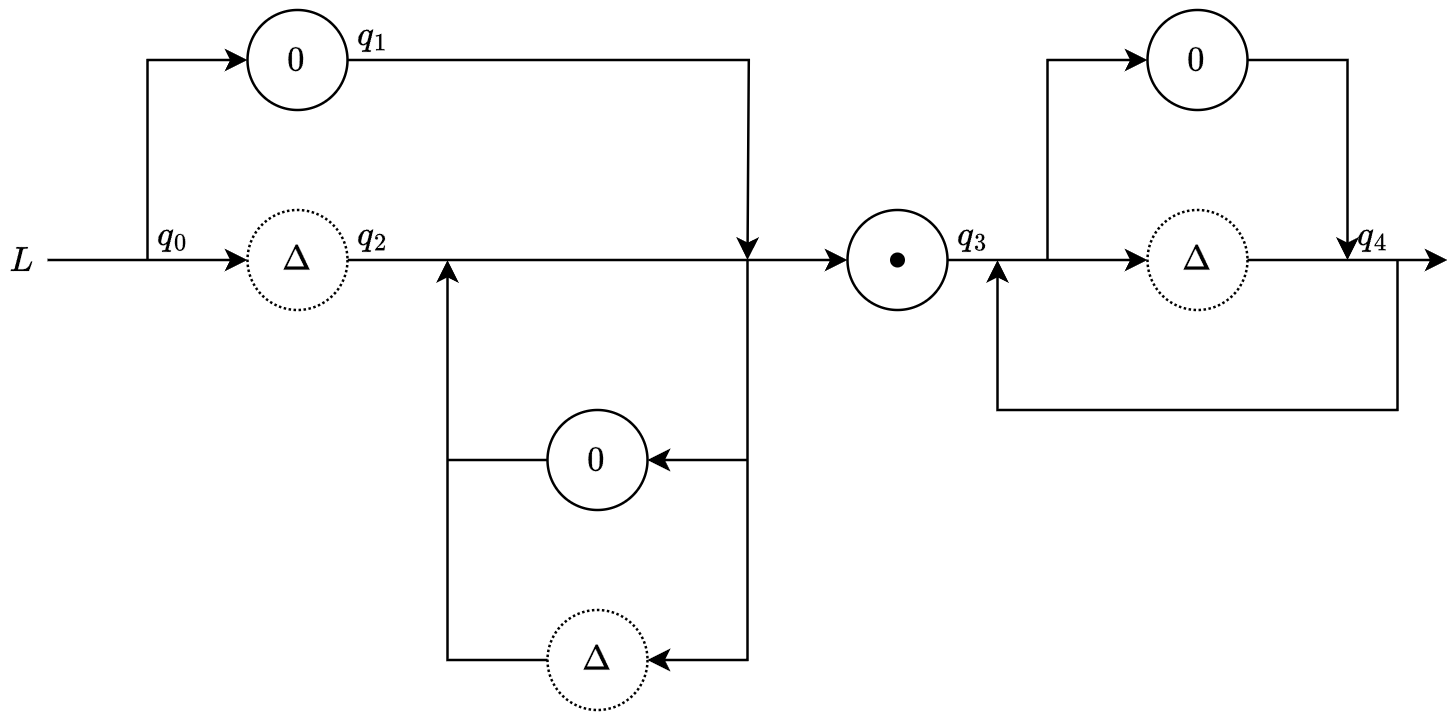
\includegraphics[width=0.75\linewidth]{images/fsa2.png}
    \end{figure}
\end{example}